% #######################################
% ########### FILL THESE IN #############
% #######################################
\def\mytitle{8x1 MULTIPLEXER}
\def\mykeywords{}
\def\myauthor{Pratheek Darla}
\def\contact{darlapratheek@gmail.com}
\def\mymodule{}
% #######################################
% #### YOU DON'T NEED TO TOUCH BELOW ####
% #######################################
\documentclass[10pt, a4paper]{article}
\usepackage[a4paper,outer=1.5cm,inner=1.5cm,top=1.75cm,bottom=1.5cm]{geometry}
\twocolumn
\usepackage{graphicx}
\graphicspath{{./images/}}
%colour our links, remove weird boxes
\usepackage[colorlinks,linkcolor={black},citecolor={blue!80!black},urlcolor={blue!80!black}]{hyperref}
%Stop indentation on new paragraphs
\usepackage[parfill]{parskip}
%% Arial-like font
\usepackage{lmodern}
\renewcommand*\familydefault{\sfdefault}
%Napier logo top right
\usepackage{watermark}
%Lorem Ipusm dolor please don't leave any in you final report ;)
\usepackage{circuitikz}
\usetikzlibrary{calc}
\usepackage{tikz}

\usetikzlibrary{shapes, arrows, chains, decorations.markings,intersections,calc}
\usepackage{lipsum}
\usepackage{xcolor}
\usepackage{listings}
%give us the Capital H that we all know and love
\usepackage{float}
%tone down the line spacing after section titles
\usepackage{titlesec}
%Cool maths printing
\usepackage{amsmath}
\usepackage{tabularx}
%PseudoCode
\usepackage{algorithm2e}

\titlespacing{\subsection}{0pt}{\parskip}{-3pt}
\titlespacing{\subsubsection}{0pt}{\parskip}{-\parskip}
\titlespacing{\paragraph}{0pt}{\parskip}{\parskip}
\newcommand{\figuremacro}[5]{
    \begin{figure}[#1]
        \centering
        \includegraphics[width=#5\columnwidth]{#2}
        \caption[#3]{\textbf{#3}#4}
        \label{fig:#2}
    \end{figure}
}

\lstset{
frame=single, 
breaklines=true,
columns=fullflexible
}

%\thiswatermark{\centering %\put(20,-80.0){\includegraphics[scale=0.4]{iith}} }
\title{\mytitle}
  \author{\myauthor\hspace{1em}\\\contact\\IITH-Future Wireless Communications(FWC22091)\hspace{0.5em}-\hspace{0.5em}\mymodule}
\date{}
\hypersetup{pdfauthor=\myauthor,pdftitle=\mytitle,pdfkeywords=\mykeywords}
\sloppy
% #######################################
% ########### START FROM HERE ###########
% #######################################
\begin{document}
	\maketitle
     \tableofcontents 
	
	  \paragraph{Abstarct-The objective of this manual is to show how to implement the Boolean function - Q = B.C + A.B.D' + A'.C'.D  in a 8x1 multiplexer. }  
	
\vspace{10mm}    
	\textbf{}{\mykeywords}
\vspace{10mm}    


    \section{Introduction}
	
    \paragraph{Mutiplexer}
    is a combinational  logic circuit designed to switch one  of  the several  inputs lines through a single common output line by the application of a control signal.
      \\ The implementation of multiplexer takes three steps\\1.To get the truth table of multiplexer\\2.To get the Boolean equation using the truth table by using k map.\\3.Then, by using the above Boolean Equation,construct circuit diagram
      \vspace{10mm}
      
      \section{Components}
     
       \begin{tabularx}{0.35\textwidth} { 
  | >{\raggedright\arraybackslash}X 
  | >{\centering\arraybackslash}X 
  | >{\raggedleft\arraybackslash}X | }
\hline
\textbf{Component} &  \textbf{Value} & \textbf{Quantity}\\
\hline
Arduino & UNO & 1 \\  
\hline
Resistor& 220ohm & 1 \\ 
\hline
Bread board & - & 1 \\
\hline
Jumber wires & M-M & 20\\
\hline
Led & - & 1\\
\hline
\end{tabularx}
\begin{center}
    Figure-1 Components
\end{center}
       \subsection{Arduino} \vspace{5mm}
      The Arduino Uno has some ground pins, analog input pins A0-A3 and digital pins D1-D13 that can be used for both input as well as output. It also has two power pins that can generate 3.3V and 5V.In the following exercises, only the ground, 5V and digital pins will be used.
\vspace{10mm}    
      
    \section{Truth Table of 8x1 Multiplexer}
        The truth table for 8x1 Multiplexer is as follows: \\Selection lines= A,B,C
	
 \begin{tabularx}{0.35\textwidth} { 
  | >{\raggedright\arraybackslash}X 
  | >{\raggedright\arraybackslash}X 
  | >{\raggedright\arraybackslash}X 
  | >{\centering\arraybackslash}X |}
\hline
 C & B & A & Q \\
\hline
 0 & 0 & 0 & I1\\  
\hline
 0 & 0 & 1 & I2  \\ 
\hline
 0 & 1 & 0 & I3 \\
\hline
 0 & 1 & 1 & I4\\
\hline
 1 & 0 & 0 & I5\\
\hline
1 & 0 & 1 & I6\\
\hline
 1 & 1 & 0 & I7\\
\hline
1 & 1 & 1 & I8\\
\hline
\end{tabularx}
\begin{center}
    Figure-2 Truth table
\end{center} 
       Building the Boolean equation:\\By using the above truth table, K-map we get the above equation as:\\Y=C'B'A'I1 + C'B'AI2 + C'BA'I3 + C'BAI4 + CB'A'I5 + CB'AI6 + CBA'I7 + CBAI8
\vspace{10mm}    
       
	\section{Circuit Diagram}
	Using the above Boolean Equation the circuit diagram is drawn as:
    \begin{center}

\vspace{10mm}    

\begin{circuitikz} \draw

(0,14) node[and port,number inputs=4]  (and1) {}
(0,12) node[and port,number inputs=4]  (and2) {}
(0,10) node[and port,number inputs=4]  (and3) {}
(0,8) node[and port,number inputs=4]  (and4) {}
(0,6) node[and port,number inputs=4]  (and5) {}
(0,4) node[and port,number inputs=4]  (and6) {}
(0,2) node[and port,number inputs=4]  (and7) {}
(0,0) node[and port,number inputs=4]  (and8) {}
(4.5,7) node[or port, number inputs=8] (or) {}
(and1.out) -- (or.in 1)
(and2.out) -- (or.in 2)
(and3.out) -- (or.in 3)
(and4.out) -- (or.in 4)
(and5.out) -- (or.in 5)
(and6.out) -- (or.in 6)
(and7.out) -- (or.in 7)
(and8.out) -- (or.in 8);
\node[left] at (and1.in 1) {\(I[1]\)};
\node[left] at (and1.in 2) {\(A\)};
\node[left] at (and1.in 3) {\(B\)};
\node[left] at (and1.in 4) {\(C\)};
\node[left] at (and1.in 2)[ocirc] {};
\node[left] at (and1.in 3)[ocirc] {};
\node[left] at (and2.in 1) {\(I[2]\)};
\node[left] at (and2.in 2) {\(A\)};
\node[left] at (and2.in 3) {\(B\)};
\node[left] at (and2.in 4) {\(C\)};
\node[left] at (and2.in 2)[ocirc] {};
\node[left] at (and3.in 1) {\(I[3]\)};
\node[left] at (and3.in 2) {\(A\)};
\node[left] at (and3.in 3) {\(B\)};
\node[left] at (and3.in 4) {\(C\)};
\node[left] at (and3.in 3)[ocirc] {};
\node[left] at (and4.in 1) {\(I[4]\)};
\node[left] at (and4.in 2) {\(A\)};
\node[left] at (and4.in 3) {\(B\)};
\node[left] at (and4.in 4) {\(C\)};
\node[right] at (or.out) {\(Q(Output)\)};
\node[left] at (and5.in 1) {\(I[5]\)};
\node[left] at (and5.in 2) {\(A\)};
\node[left] at (and5.in 3) {\(B\)};
\node[left] at (and5.in 4) {\(C\)};
\node[right] at (or.out) {\(Q(Output)\)};
\node[left] at (and6.in 1) {\(I[6]\)};
\node[left] at (and6.in 2) {\(A\)};
\node[left] at (and6.in 3) {\(B\)};
\node[left] at (and6.in 4) {\(C\)};
\node[right] at (or.out) {\(Q(Output)\)};
\node[left] at (and7.in 1) {\(I[7]\)};
\node[left] at (and7.in 2) {\(A\)};
\node[left] at (and7.in 3) {\(B\)};
\node[left] at (and7.in 4) {\(C\)};
\node[right] at (or.out) {\(Q(Output)\)};
\node[left] at (and8.in 1) {\(I[8]\)};
\node[left] at (and8.in 2) {\(A\)};
\node[left] at (and8.in 3) {\(B\)};
\node[left] at (and8.in 4) {\(C\)};
\node[right] at (or.out) {\(Q(Output)\)};
\end{circuitikz}







        
    \end{center}

\begin{center}
    
\vspace{10mm}    

 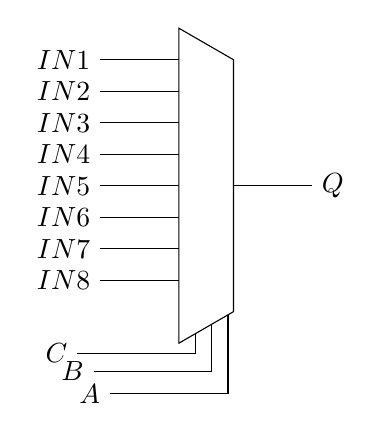
\begin{tikzpicture}

    \draw[scale=0.8] 
                (90,8)coordinate (O)
            --++(30:1)coordinate (A)
            --++(90:4)coordinate (B)
            --++(150:1) coordinate (C)
            --cycle;
        \draw ($(A)!0.5!(B)$)--++(0:1)node[right]{$Q$};

    \draw ($(O)!0.9!(A)$)--++(-90:1)--++(180:1.5)node[left]{$A$};

    \draw ($(O)!0.3!(A)$)--++(-90:0.25)--++(180:1.5)node[left]{$C$};
    \draw ($(O)!0.6!(A)$)--++(-90:0.6)--++(180:1.5)node[left]{$B$};

    \foreach \y/\t in {0.1/1,0.2/2,0.3/3,0.4/4,0.5/5,0.6/6,0.7/7,0.8/8} {
    \draw ($(C)! \y*1 !(O)$)--++(180:1) node[left] {$IN \t$};}      

    \end{tikzpicture}
    \\ Figure- 8:1 multiplexer
\end{center}

\vspace{10mm}    

\section{Hardware}
1. Connect Arduino to the computer and upload the code in to the Arduino. Make 2,3,4,5 pins as input pins and 13 pin as output pin. Corresponds to the given inputs for the selection lines of multiplexer the outputs will be obtained at 13 pin. The builtin led in Arduino is the indication of the output of multiplexer.

\vspace{10mm}    
The truth table for the Boolean function - Q = B.C + A.B.D' + A'.C'.D  is given below:

\vspace{5mm}    

\begin{tabularx}{0.50\textwidth} { 
  | >{\centering\arraybackslash}X
  | >{\centering\arraybackslash}X 
  | >{\centering\arraybackslash}X 
  || >{\centering\arraybackslash}X 
  | >{\centering\arraybackslash}X 
  | >{\centering\arraybackslash}X| }
\hline
Selection
line&Selection
line&Selection line&Input &Output\\
\hline
C&  B & A & D & Q\\
\hline
0 & 0 & 0 & D & D\\  
\hline
0 & 0 & 1 & 0 & 0\\ 
\hline
0 & 1 & 0 & D & D\\
\hline
0 & 1 & 1 & D' & D'\\
\hline
1 & 0 & 0 & 0 & 0\\
\hline
1 & 0 & 1 & 0 & 0\\
\hline
1 & 1 & 0 & 1 & 1\\
\hline
1 & 1 & 1 & 1 & 1\\
\hline
\end{tabularx}

\vspace{10mm}    

\section{Software}
 Download the following code
 \begin{lstlisting}
https://github.com/PratheekDarla/FWC-IITH/blob/main/assignment/codes/src/main.cpp
 \end{lstlisting}

\end{document}